\documentclass[a4paper]{article}
\usepackage{amsfonts}
\usepackage{amsmath}
\usepackage{amssymb}
\usepackage{graphicx}     
\usepackage{cancel}

% Command definities van frequent gebruikte commandos
\newcommand{\N}{\mathbb{N}}
\newcommand{\Q}{\mathbb{Q}}
\newcommand{\R}{\mathbb{R}}
\newcommand{\C}{\mathbb{C}}
\newcommand{\Bgsin}{\operatorname{Bgsin}}
\newcommand{\Bgcos}{\operatorname{Bgcos}}
\newcommand{\Bgtan}{\operatorname{Bgtan}}
\newcommand{\cis}{\operatorname{cis}}
\newcommand{\Limit}{\lim\limits_}

\begin{document}
  
\noindent \large Auteur: Wout Vanderborght\\
\noindent \large Studierichting: Informatica\\
\noindent \large Oefeningenreeks 3H nr. 12.3\\

\medskip

\normalsize

Bestudeer de functie met de volgende poolvergelijking: \\

$ r = 3\tan(\theta) $ \\

Deze functie is periodisch met periode $\pi$ dus we beperken ons tot $\left[0, \pi\right]$. \\

Nulpunten: $\left\{0, \pi\right\}$, bestaat niet in $\dfrac{\pi}{2}$ \\

$ r' = 3\sec^2(\theta) $ \\

Nulpunten: $\emptyset$, bestaat niet in $\dfrac{\pi}{2}$ \\

\begin{tabular}{c|ccccc}
 $\theta$ & $0$ & & $\dfrac{\pi}{2}$ & & $\pi$ \\ \hline
 $r(\theta)$ & $0$ & $+$ & $|$ & $-$ & $0$ \\
 $r'(\theta)$ & $+$ & $+$ & $|^{(2)}$ & $+$ & $+$ \\ \hline
 $r(\theta)$ & $\nearrow$ & $\nearrow$ & & $\nearrow$ & $\nearrow$ \\
\end{tabular} \\

Tekening: \\

\begin{figure}[h]
\centering
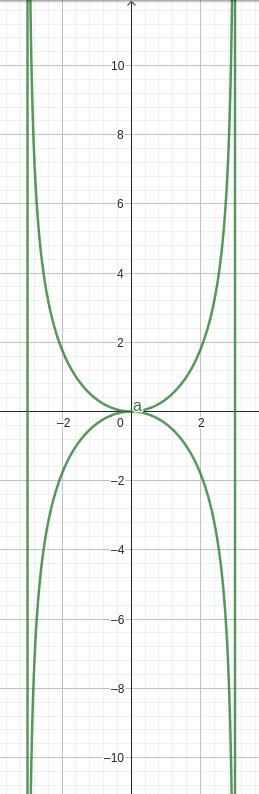
\includegraphics[width=2.7cm]{3H-12.3-wout.vanderborght.INF.png} \\
\end{figure}

\begin{thebibliography}{999}
%\bibitem{a} Referentie
\end{thebibliography}
\end{document} 
